\documentclass[12pt,a4paper]{article}
\usepackage{geometry}
\geometry{left=2.5cm,right=2.5cm,top=2.0cm,bottom=2.5cm}
\usepackage[english]{babel}
\usepackage{amsmath,amsthm}
\usepackage{amsfonts}
\usepackage{bm}
\usepackage[longend,ruled,linesnumbered]{algorithm2e}
\usepackage{siunitx}
\usepackage{fancyhdr}
\usepackage{ctex}
\usepackage{array}
\usepackage{listings}
\usepackage{color}
\usepackage{graphicx}
\usepackage{float}
\usepackage{caption}
\usepackage{longtable}

\begin{document}
    \title{\heiti{《机器学习》课程第 {$5$} 次作业}}
    \date{}
    \author{姓名:\underline{刘哲}~~~~~~学号:\underline{2022103691}~~~~~~}
    \maketitle
    \section{\heiti{第9题}}
    \vspace{10pt}
    \subsection*{a}
    三次多项式回归的结果为
    \begin{figure}[H]
        \centering
        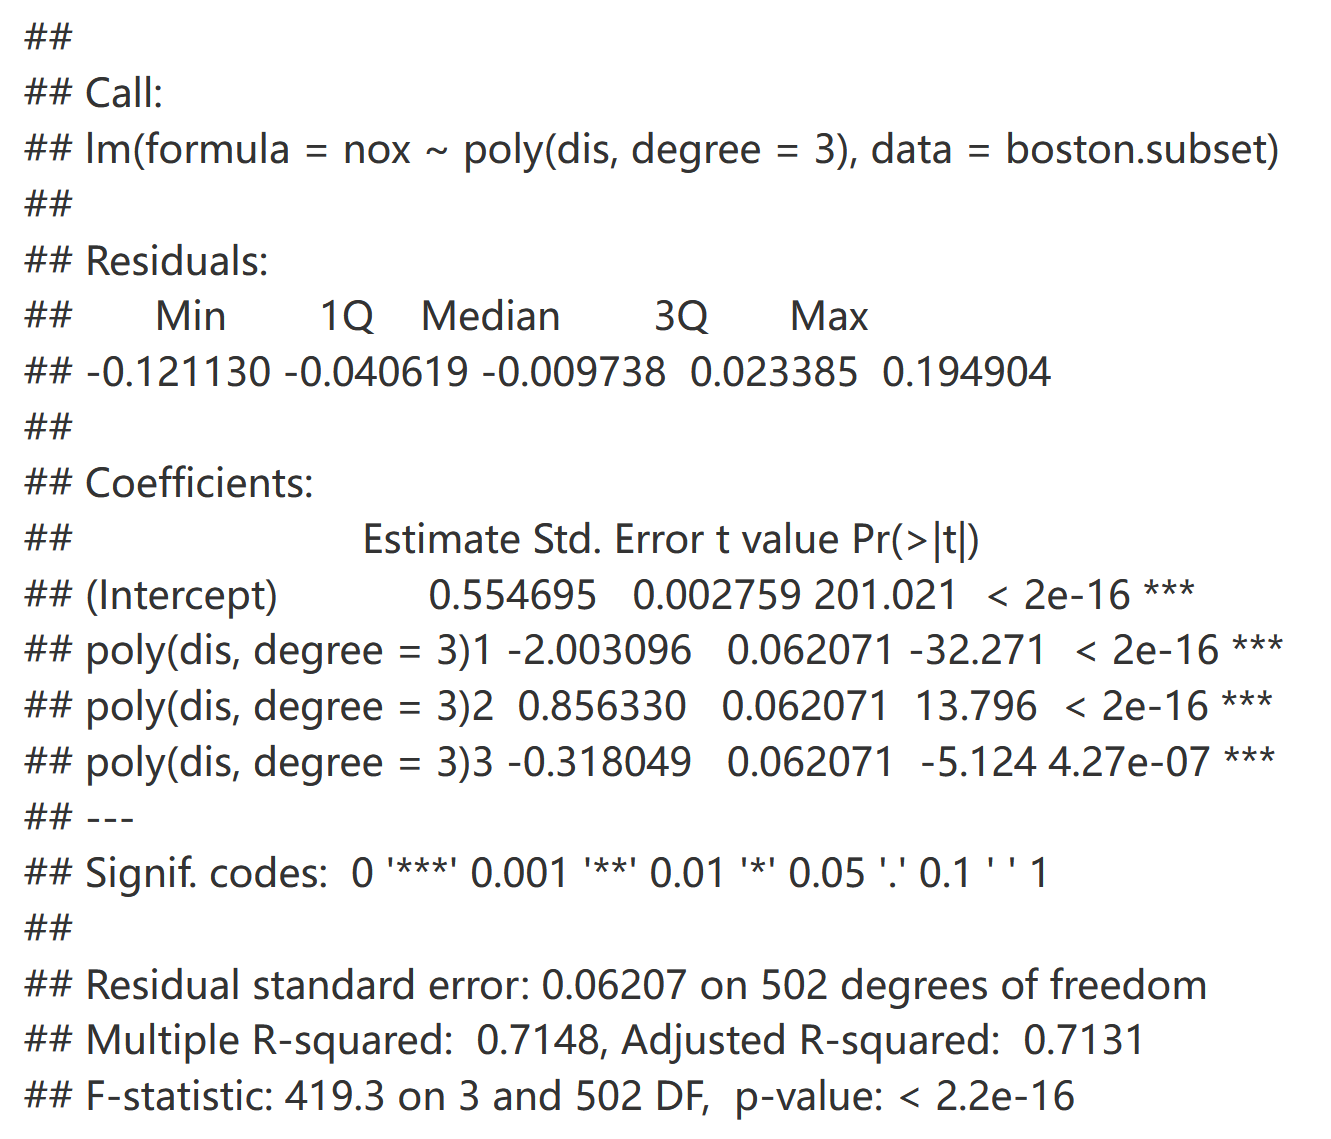
\includegraphics[scale=0.3]{CubicReg.png}
    \end{figure}
    可以看出,回归系数均显著,模型显著。三次多项式回归的拟合曲线为
    \begin{figure}[H]
        \centering
        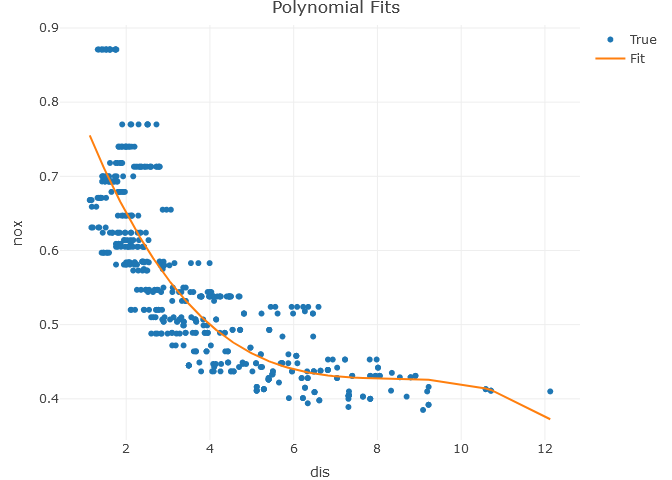
\includegraphics[scale=0.6]{CubicFit.png}
    \end{figure}
    拟合曲线在样本数据的中间位置表现尚可,但在两端表现很差,拟合曲线出现了对样本数据明显的偏离。
    \subsection*{b}
    选取多项式回归的 $degree$ 为 $1\sim 10$,分别进行多项式回归,拟合曲线分别为
    \begin{figure}[H]
        \centering
        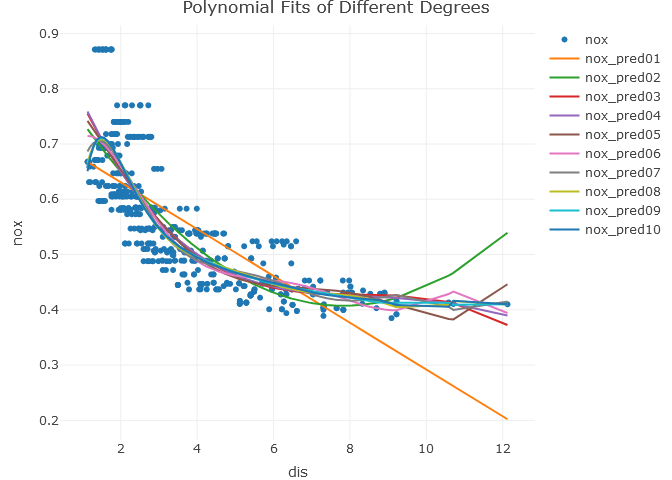
\includegraphics[scale=0.6]{PolyDeg.png}
    \end{figure}
    计算各个回归模型的 $RSS$ 为
    \begin{longtable}{c|c|c|c|c|c}
        \hline
        Degree & 1 & 2 & 3 & 4 & 5\\
        \hline
        RSS & 2.7686 & 2.0353 & 1.9341 & 1.9330 & 1.9153\\
        \hline
        \hline
        Degree & 6 & 7 & 8 & 9 & 10\\
        \hline
        RSS & 1.8783 & 1.8495 & 1.8356 & 1.8333 & \textbf{1.8322}\\
        \hline
    \end{longtable}
    根据结果可知,当 $degree=10$ 时,多项式回归模型具有最小的 $RSS$,但此时可能存在比较严重的过拟合问题。
    拟合曲线为
    \begin{figure}[H]
        \centering
        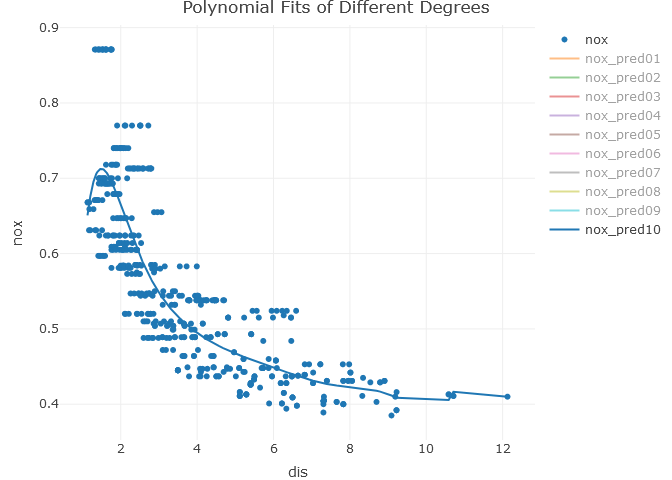
\includegraphics[scale=0.6]{Poly10Fit.png}
    \end{figure}
    \subsection*{c}
    为了降低发生过拟合的可能性,使用十折交叉验证的方法训练每个 $degree$ 下的多项式回归模型。
    将样本数据随机平均分为 $10$ 组,在每个 $degree$ 下,每次选择一组数据作为验证集,其余九组作为训练集训练模型。
    将十折验证集的 $RSS$ 加和作为该 $degree$ 的 $RSS$,结果为
    \begin{longtable}{c|c|c|c|c|c}
        \hline
        Degree & 1 & 2 & 3 & 4 & 5\\
        \hline
        RSS & 2.7889 & 2.0600 & \textbf{1.9594} & 1.9725 & 2.1317\\
        \hline
        \hline
        Degree & 6 & 7 & 8 & 9 & 10\\
        \hline
        RSS & 2.6212 & 5.2695 & 2.8932 & 3.8634 & 2.7334\\
        \hline
    \end{longtable}
    根据结果可知,当 $degree=10$ 时,多项式回归模型具有最小的 $RSS$,认为最优 $degree$ 为 $3$。
    拟合曲线见\textbf{a}。\par
    由于使用交叉验证法降低了发生过拟合的可能性,该结果较为可信。
    \subsection*{d}
    令自由度为 $4$,设 $knots$ 为变量 $dis$ 的分位数
    \begin{longtable}{c|c|c|c}
        \hline
        Quantile & 25\% & 50\% & 75\%\\
        \hline
        Value & 2.1002 & 3.2075 & 5.1884\\
        \hline
    \end{longtable}
    拟合回归样条的结果为
    \begin{figure}[H]
        \centering
        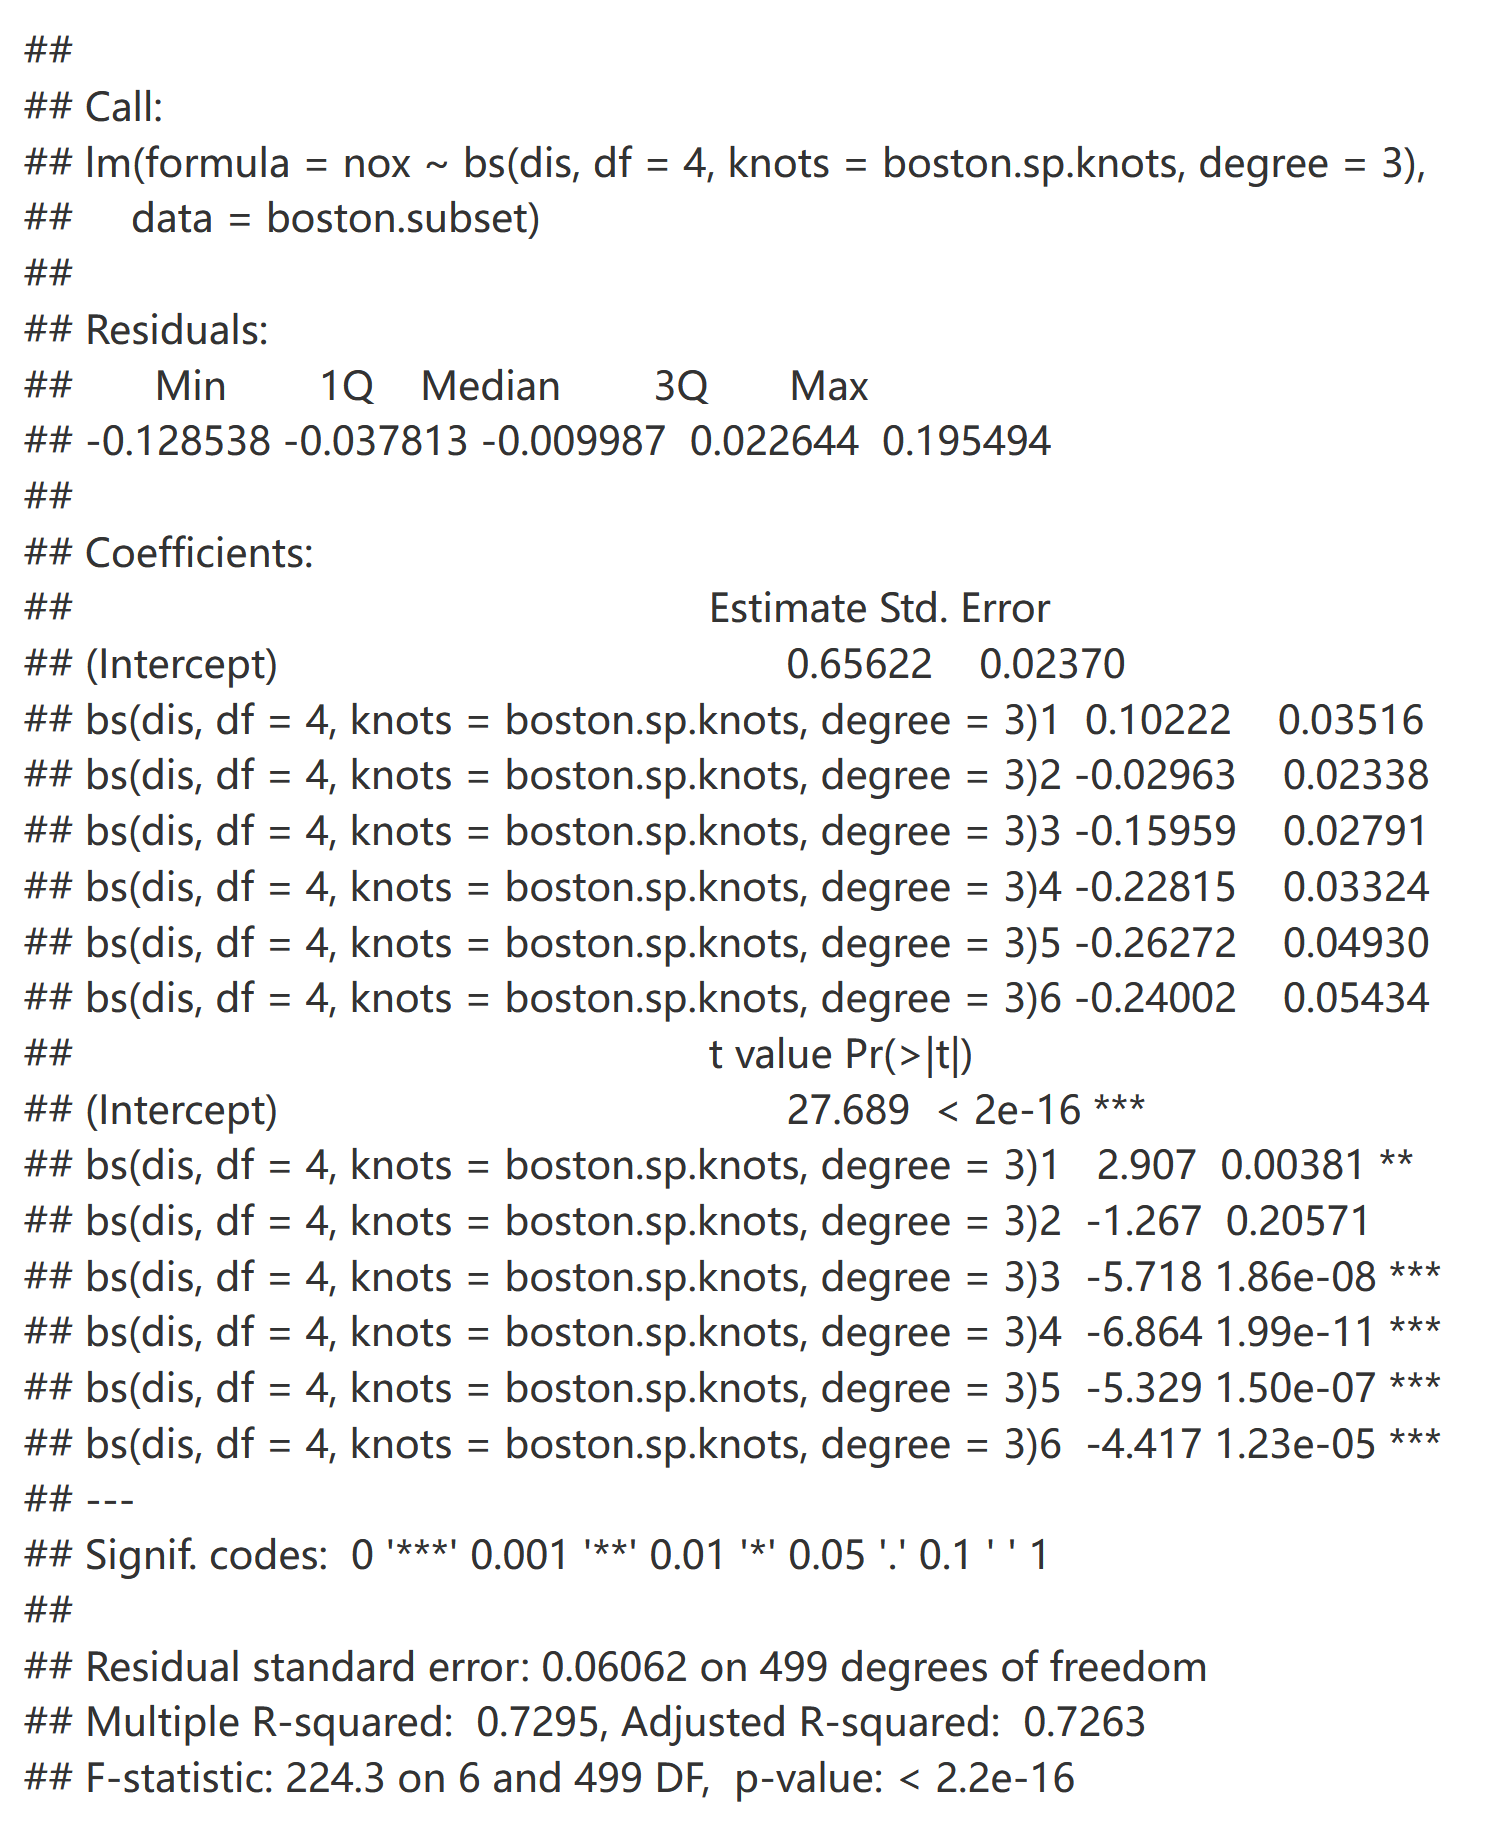
\includegraphics[scale=0.3]{RegSpline4.png}
    \end{figure}
    可以看出,不是所有回归系数都显著,但模型显著。回归样条的拟合曲线为
    \begin{figure}[H]
        \centering
        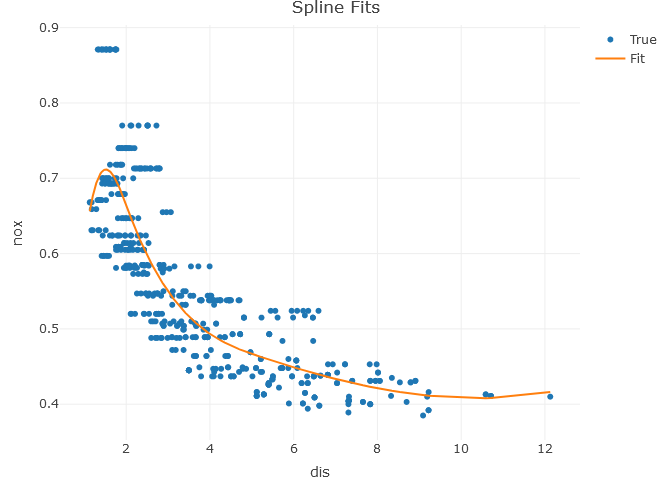
\includegraphics[scale=0.6]{RegSpline4Fit.png}
    \end{figure}
    \subsection*{e}
    选取回归样条的自由度为 $1\sim 10$,分别进行回归样条,拟合曲线分别为
    \begin{figure}[H]
        \centering
        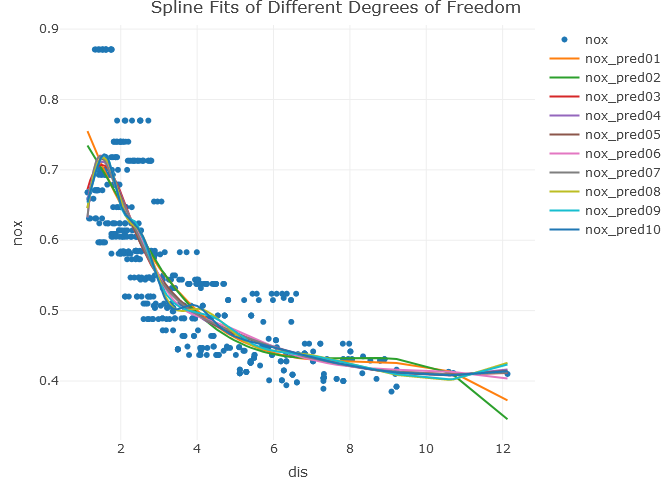
\includegraphics[scale=0.6]{RegSplineDF.png}
    \end{figure}
    计算各个回归模型的 $RSS$ 为
    \begin{longtable}{c|c|c|c|c|c}
        \hline
        DF & 1 & 2 & 3 & 4 & 5\\
        \hline
        RSS & 1.9341 & 1.9228 & 1.8402 & 1.8340 & 1.8299\\
        \hline
        \hline
        DF & 6 & 7 & 8 & 9 & 10\\
        \hline
        RSS & 1.8170 & 1.8257 & 1.7925 & 1.7970 & \textbf{1.7890}\\
        \hline
    \end{longtable}
    根据结果可知,当 $DF=10$ 时,回归样条模型具有最小的 $RSS$,但此时可能存在过拟合问题。
    拟合曲线为
    \begin{figure}[H]
        \centering
        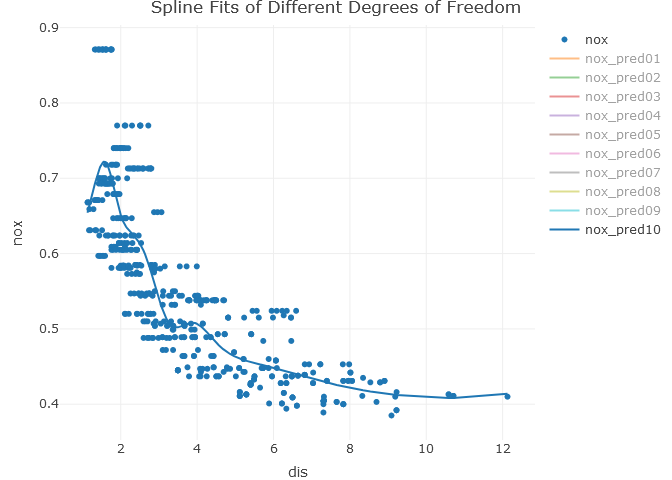
\includegraphics[scale=0.6]{RegSpline10Fit.png}
    \end{figure}
    \subsection*{f}
    为了降低发生过拟合的可能性,使用十折交叉验证的方法训练每个 $DF$ 下的回归样条模型。
    将样本数据随机平均分为 $10$ 组,在每个 $DF$ 下,每次选择一组数据作为验证集,其余九组作为训练集训练模型。
    将十折验证集的 $RSS$ 加和作为该 $DF$ 的 $RSS$,结果为
    \begin{longtable}{c|c|c|c|c|c}
        \hline
        DF & 1 & 2 & 3 & 4 & 5\\
        \hline
        RSS & 1.9594 & 1.9747 & 1.8741 & 1.8754 & 1.8743\\
        \hline
        \hline
        DF & 6 & 7 & 8 & 9 & 10\\
        \hline
        RSS & 1.8646 & 1.8765 & \textbf{1.8633} & 1.8744 & 1.8651\\
        \hline
    \end{longtable}
    根据结果可知,当 $DF=8$ 时,回归样条模型具有最小的 $RSS$,认为最优 $DF$ 为 $8$。
    拟合曲线为
    \begin{figure}[H]
        \centering
        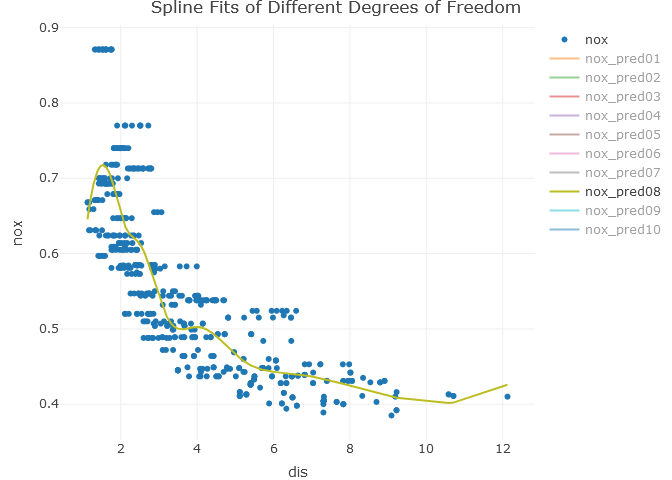
\includegraphics[scale=0.6]{RegSpline8Fit.png}
    \end{figure}
    由于使用交叉验证法降低了发生过拟合的可能性,该结果较为可信。
\end{document}